\documentclass[tikz, border=10pt]{standalone}
\usepackage[T1]{fontenc}
\usepackage[utf8]{inputenc}
\usepackage{lmodern}
\usepackage[table]{xcolor}
\definecolor{IntelBlue}{HTML}{0068B5}
\definecolor{IntelLightBlue}{HTML}{DDEEF9}
\definecolor{FpgaOrange}{HTML}{E67E22}
\definecolor{FpgaLight}{HTML}{FDEBD0}
\definecolor{HpsGreen}{HTML}{1A7A4A}
\definecolor{HpsLight}{HTML}{D5F5E3}
\definecolor{GrayBg}{HTML}{F2F3F4}
\definecolor{GrayBorder}{HTML}{AAB7B8}
\definecolor{PassGreen}{HTML}{D5F5E3}
\definecolor{PassGreenDark}{HTML}{1E8449}
\definecolor{RowAlt}{HTML}{F7F9FB}
\definecolor{SummaryBg}{HTML}{EBF5FB}
\definecolor{NodeFill}{HTML}{D6EAF8}
\definecolor{NodeBorder}{HTML}{1B4F72}
\definecolor{InitFill}{HTML}{E5E7E9}
\definecolor{InitBorder}{HTML}{717D7E}
\definecolor{SleepFill}{HTML}{FEF5E7}
\definecolor{SleepBorder}{HTML}{935116}
\definecolor{MsgFill}{HTML}{D1F2EB}
\definecolor{MsgBorder}{HTML}{0E6655}
\definecolor{TimeoutRed}{HTML}{C0392B}
\definecolor{BtnBlue}{HTML}{1A5276}
\definecolor{ArrowGray}{HTML}{717D7E}
\usepackage{tikz}
\usetikzlibrary{shapes.geometric, arrows.meta, positioning, fit, backgrounds, calc, decorations.pathreplacing, bending, shadows.blur}
\begin{document}
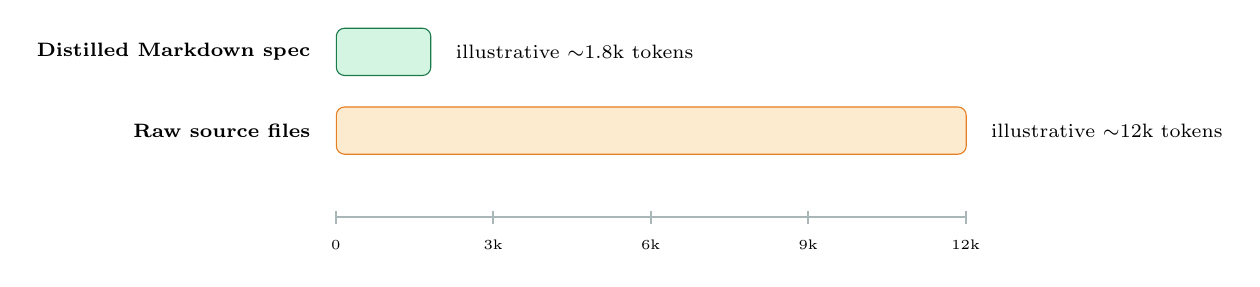
\begin{tikzpicture}[
  axis/.style={draw=GrayBorder, line width=0.8pt},
  bar/.style={rectangle, rounded corners=3pt, minimum height=0.6cm,
              anchor=west},
  lbl/.style={font=\scriptsize\bfseries, anchor=east},
  val/.style={font=\scriptsize, anchor=west},
]
\draw[axis] (0,0) -- (8,0);
\foreach \x/\n in {0/0,2/3k,4/6k,6/9k,8/12k} {
  \draw[axis] (\x,0.08) -- (\x,-0.08);
  \node[font=\tiny] at (\x,-0.35) {\n};
}
\node[lbl] at (-0.2,1.1) {Raw source files};
\node[bar, fill=FpgaLight, draw=FpgaOrange, minimum width=8cm] at (0,1.1) {};
\node[val] at (8.2,1.1) {illustrative $\sim$12k tokens};

\node[lbl] at (-0.2,2.1) {Distilled Markdown spec};
\node[bar, fill=HpsLight, draw=HpsGreen, minimum width=1.2cm] at (0,2.1) {};
\node[val] at (1.4,2.1) {illustrative $\sim$1.8k tokens};
\end{tikzpicture}
\end{document}
